\documentclass[tikz,border=5mm]{standalone}
\usetikzlibrary{matrix, positioning}

\begin{document}
    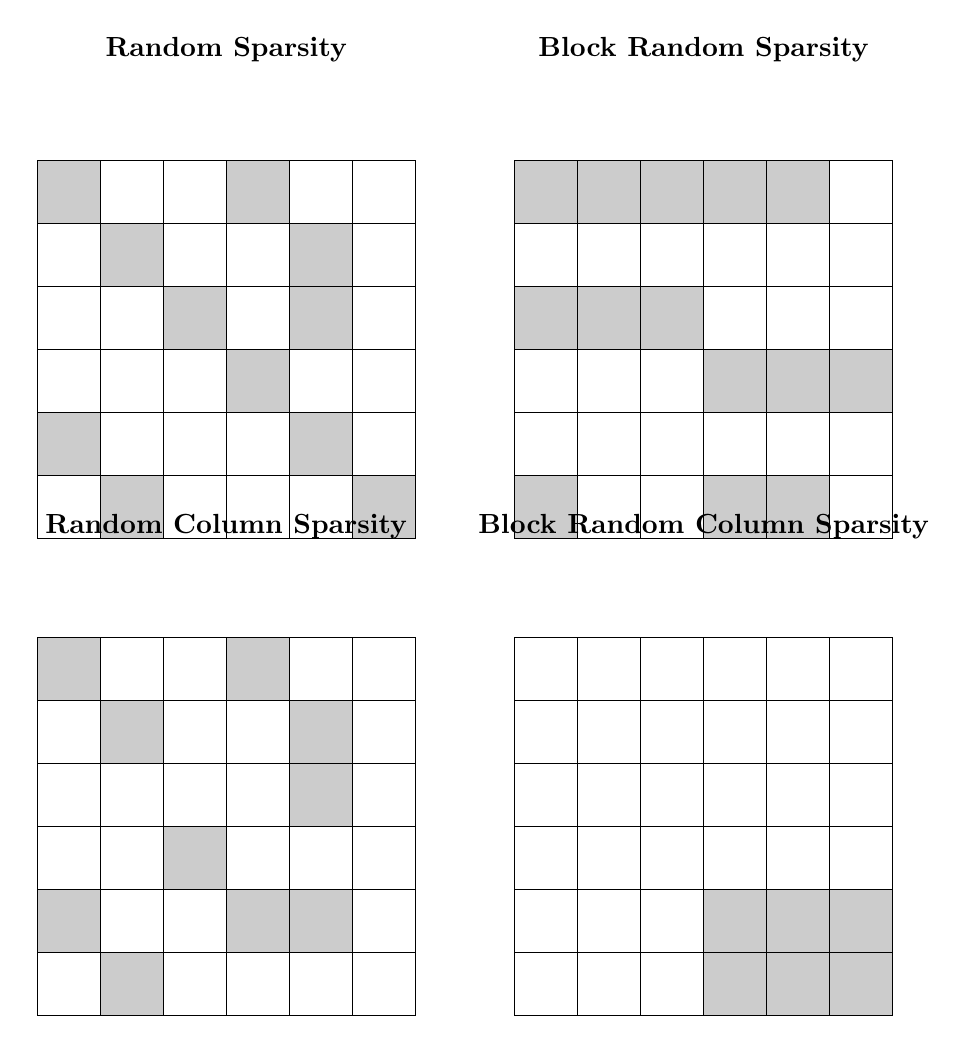
\begin{tikzpicture}[scale=0.6]
        
        % Define styles for the matrix nodes
        \tikzset{
            filled/.style={fill=gray!40},
            unfilled/.style={fill=white},
            mymatrix/.style={
                matrix of nodes,
                nodes in empty cells,
                column sep=-\pgflinewidth,
                row sep=-\pgflinewidth,
                nodes={
                    minimum size=8mm,
                    draw=black,
                    anchor=center,
                    inner sep=0pt,
                }
            },
        }

        % Random Sparsity Matrix
        \matrix[mymatrix] (random_matrix) at (-7,0) {
            |[filled]| & |[unfilled]| & |[unfilled]| & |[filled]| & |[unfilled]| & |[unfilled]| \\
            |[unfilled]| & |[filled]| & |[unfilled]| & |[unfilled]| & |[filled]| & |[unfilled]| \\
            |[unfilled]| & |[unfilled]| & |[filled]| & |[unfilled]| & |[filled]| & |[unfilled]| \\
            |[unfilled]| & |[unfilled]| & |[unfilled]| & |[filled]| & |[unfilled]| & |[unfilled]| \\
            |[filled]| & |[unfilled]| & |[unfilled]| & |[unfilled]| & |[filled]| & |[unfilled]| \\
            |[unfilled]| & |[filled]| & |[unfilled]| & |[unfilled]| & |[unfilled]| & |[filled]| \\
        };
        \node[above=1cm of random_matrix] {\textbf{Random Sparsity}};

        % Block Random Sparsity Matrix
        \matrix[mymatrix, right=of random_matrix] (block_random_matrix) {
            |[filled]| & |[filled]| & |[filled]| & |[filled]| & |[filled]| & |[unfilled]| \\
            |[unfilled]| & |[unfilled]| & |[unfilled]| & |[unfilled]| & |[unfilled]| & |[unfilled]| \\
            |[filled]| & |[filled]| & |[filled]| & |[unfilled]| & |[unfilled]| & |[unfilled]| \\
            |[unfilled]| & |[unfilled]| & |[unfilled]| & |[filled]| & |[filled]| & |[filled]| \\
            |[unfilled]| & |[unfilled]| & |[unfilled]| & |[unfilled]| & |[unfilled]| & |[unfilled]| \\
            |[filled]| & |[unfilled]| & |[unfilled]| & |[filled]| & |[filled]| & |[unfilled]| \\
        };
        \node[above=1cm of block_random_matrix] {\textbf{Block Random Sparsity}};

        % Random Column Sparsity Matrix
        \matrix[mymatrix, below=of random_matrix] (random_column_matrix) {
            |[filled]| & |[unfilled]| & |[unfilled]| & |[filled]| & |[unfilled]| & |[unfilled]| \\
            |[unfilled]| & |[filled]| & |[unfilled]| & |[unfilled]| & |[filled]| & |[unfilled]| \\
            |[unfilled]| & |[unfilled]| & |[unfilled]| & |[unfilled]| & |[filled]| & |[unfilled]| \\
            |[unfilled]| & |[unfilled]| & |[filled]| & |[unfilled]| & |[unfilled]| & |[unfilled]| \\
            |[filled]| & |[unfilled]| & |[unfilled]| & |[filled]| & |[filled]| & |[unfilled]| \\
            |[unfilled]| & |[filled]| & |[unfilled]| & |[unfilled]| & |[unfilled]| & |[unfilled]| \\
        };
        \node[above=1cm of random_column_matrix] {\textbf{Random Column Sparsity}};

        % Block Random Column Sparsity Matrix
        \matrix[mymatrix, below=of block_random_matrix] (block_random_column_matrix) {
            |[unfilled]| & |[unfilled]| & |[unfilled]| & |[unfilled]| & |[unfilled]| & |[unfilled]| \\
            |[unfilled]| & |[unfilled]| & |[unfilled]| & |[unfilled]| & |[unfilled]| & |[unfilled]| \\
            |[unfilled]| & |[unfilled]| & |[unfilled]| & |[unfilled]| & |[unfilled]| & |[unfilled]| \\
            |[unfilled]| & |[unfilled]| & |[unfilled]| & |[unfilled]| & |[unfilled]| & |[unfilled]| \\
            |[unfilled]| & |[unfilled]| & |[unfilled]| & |[filled]| & |[filled]| & |[filled]| \\
            |[unfilled]| & |[unfilled]| & |[unfilled]| & |[filled]| & |[filled]| & |[filled]| \\
        };
        \node[above=1cm of block_random_column_matrix] {\textbf{Block Random Column Sparsity}};

    \end{tikzpicture}
\end{document}